\chapter{Introducción} %

%El esqueleto teórico de la física de estado sólido esta construido en dos principales pilares: el electromagnetismo y la mecánica cuántica. El primero describe las fuerzas de interacción entre los entre los electrones y el núcleo, y el segundo describe los estados energéticos accesibles del sistema, ambas ramas de la física son necesarias para describir las propiedades macroscópicas de la materia en estado sólido. Sin embargo las diferencias clásicas y no clásicas entre las teorías, generan detalles en las definiciones fundamentales como lo es en la polarización \cite{Shore2018}.%


La descripción del comportamiento de los electrones en el estado sólido esta construido en dos pilares de la física: el electromagnetismo y la mecánica cuántica. El primero describe las fuerzas de interacción entre los entre los electrones y el núcleo, y el segundo describe los estados energéticos accesibles del sistema, ambas ramas de la física son necesarias para describir sus propiedades macroscópicas. Sin embargo las diferencias clásicas y no clásicas entre las teorías, generan detalles en las definiciones fundamentales, por ejemplo en la polarización \cite{Shore2018}.


%\comA{Me parece que el siguiente párrafo no se entiende, a lo mejor con la inclusión de una figura es suficiente. La problemática de la definición de la polarización es el operador de posición, el cual depende de la elección del origen, y en el caso de tener una celda con simetría de traslación puede dar resultados muy diferentes.}
Clásicamente la polarización es la suma de momentos dipolares en una celda dividida entre el volumen de la celda, esto considera que las contribuciones de las cargas están identificadas en localizables {\it centros de polarización} [Fig. \ref{fig:cell_selection} \textbf{(a)}]. Sin embargo esto no pasa en los sólidos reales, en estos casos, la carga eléctrica que propicia la polarización tiene una distribución de probabilidad sobre todo el material que no puede ser localizada sin ambigüedad en celdas especificas [Fig. \ref{fig:cell_selection} \textbf{(b)}]. Este detalle es tan significativo que puede generar diferencias de hasta un orden de magnitud entre la polarización medida y la calculada, como lo es en el caso del silicio \cite{rabe2007modern}.\comA{Esta última referencia sería mejor que fuera más específica, es un dato muy puntual para mandar de referencia a un libro.}


\begin{figure}[h!]
    \centering
   \captionsetup[sub]{font=small}

    \begin{subfigure}[b!]{0.3 \textwidth}
        \caption{}\vspace*{0.5em}
        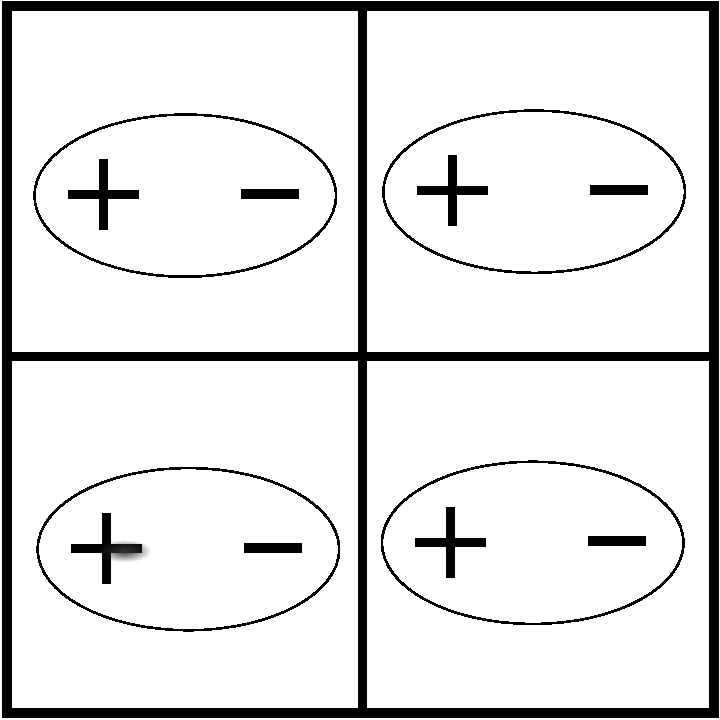
\includegraphics[width=\textwidth]{Imagenes/no_cell_selection.pdf}
    \end{subfigure}\hspace*{2em}
    \begin{subfigure}[b!]{0.3 \textwidth}
        \caption{}\vspace*{0.5em}
        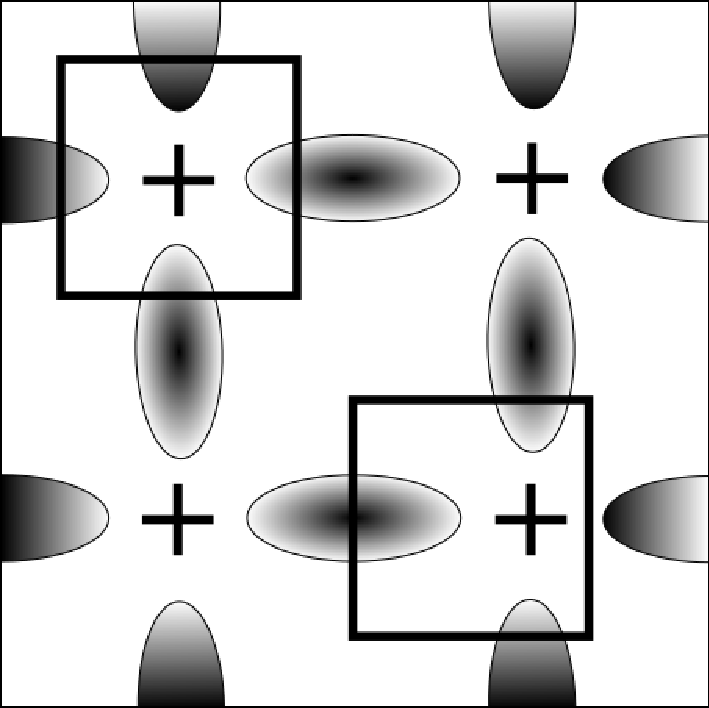
\includegraphics[width=\textwidth]{Imagenes/Cell_selection.pdf}
    \end{subfigure}\hspace*{1em} \vspace*{0.5em}
       \caption{\textbf{(a)} Selección de celdas en la polarización clasica donde se asumen los dipolos como unidades empquetadas. \textbf{(b)} Selección arbitraria de celda para calcular el momento dipolar cuando la densidad electronica esta distribuida por todo el aislante.}.
       \label{fig:cell_selection}
\end{figure}

Con el fin de solucionar estos problemas fue necesaria una nueva teoría que es conocida como ''\textit{Teoría moderna de la polarización}'' o ''\textit{Teoría de la fase de Berry de la polarización}'' introducida en 1990 por \textit{Resta, king-Smith} y \textit{Vanderbilt} en 1990. Esta teoría propone calcular la polarización por medio de las contribuciones de las fases de la función de onda, llamada fase de Berry. Esta teoría da una novedosa solución a los problemas de multivalución de la polarización en sistemas infinitos \cite{spaldin2012beginner}, las diferencias entre los cálculos teóricos y experimentales de las contribuciones de borde en la polarización en dieléctricos \cite{rabe2007modern}, la aparición de fases topológicas en la cadena de poliacetileno como lo es el bombeo de Thouless \comA{Cita Thouless pump} y en los últimos años a permitido la clasificación de fases topológicas de orden superior, como la aparición de multipolos eléctricos cuantizados en redes cuadradas \cite{Benalcazar2017}. Siendo, estas ultimas dos referencias, la inspiración de este trabajo.  


{\it Las fases topológicas en los sólidos.---} El primer ejemplo de materiales que presentan una fase topológica son los aislantes topológicos. Los aislantes topológicos o TIs (Topological Insulators) son materiales con una fase electrónica no convencional, los cuales se diferencian de los aislantes ordinarios en que aunque sus electrones no conducen en el cuerpo del material; pero, las superficies para un arreglo tridimensional o las aristas para un arreglo bidimensional mantienen estados metálicos o de conducción protegidos por una simetría de inversión del tiempo o TRS (time-reversal symmetry) \cite{Shore2018}. La exitosa predicción estos nuevos materiales (TIs), es tal vez el triunfo mas espectacular de la teoría moderna de bandas, basada en primeros principios \comA{(Hohenberg and Kohn 1964; Kohn and Sham 1965). buscar estas citas} 

La simetría especial que protege los estados electrónicos en los TIs genera prometedoras expectativas  en la creación de nuevas plataformas para el estudio de preguntas fundamentales en la ciencia, como lo son las nuevas texturas del spin y exóticos estados de superconductividad,  así como la realización de dispositivos topológicos multifunciones que tienen una serie de aplicaciones en la termoeléctrica, spintrónica, procesamiento de información, etc. Además en los TIs son posibles varios fenómenos cuánticos muy exóticos, por ejemplo, los fermiones de Majonara, axiones, monopolos magnéticos, excitaciones fracciónales, que no se pueden trabajar sobre la base de los primeros principios \cite{Moore2010}.

Matemáticamente se dice dos aislantes pertenece a la misma clase topológica si y solo si sus Hamiltonianos pueden estar continuamente conectados, en el sentido de que la brecha nunca debe cerrarse en ningún punto a lo largo del camino que los conecta. Es posible hacer una analogía con la clasificación topológica de las superficies geométricas cerradas, por ejemplo, se dice que dos superficies son topológicamente equivalentes si se puede pasar de una a la otra sin ningún ``evento violento'' en la transformación, como abrir nuevos agujeros o cerrar los viejos. En la clasificación de estos estados encontraremos que un cristal aislante es ``\textit{trivial}'' si puede ser conectado adiabáticamente sin cerrar la brecha en un limite atómico y que es \textit{topológico} si no cumple esto.

Sin embargo, una nueva clasificación de los TIs ha aparecido en le desarrollo del estudio de los multipolos eléctricos aislantes cuantizados hecho por Benalcazar et al. \cite{Benalcazar2017}    en el que se generaliza la relación cuerpo-frontera (bulk-bundary). En el se presentan aislantes en dos y tres dimensiones, los cuales no presentan estados sin brecha en las aristas o superficie, respectivamente, sin embargo si poseen estados sin brecha (gapless) los cuales se muestran en las esquinas del cristal, estas excitaciones topológicas en las esquinas corresponden a momentos multipolares cuantizados.
La topología del cuerpo el cual contiene estados protegidos, sin brecha en las aristas o aristas y con brecha en el cuerpo y la superficie, asumen un noción de lo que es un aíslate topológico de alto orden o HOTI (High Order Topological Insulator). Un TI de n-simo orden que tiene modos protegidos sin brecha en las fronteras del material de codimensión n. Actualmente se han logrado observar estos estados en arreglos fonónicos.

Como se puede notar, el comportamiento de un HOTI esta altamente relacionado con la dimensionalidad del volumen del cristal, perímetro y vértices, pero, ¿Qué pasaría si la dimensionalidad de este aislante no es entera, es decir, de dimensión fractal? ¿Los estados de polarización o transporte electrónico se mantendrían robustos en una dimensión fractal? Experimentalmente, los materiales con dimensiones fractales o no enteras pueden aparecer como resultado de un crecimiento fractal, límites aproximados y paredes de dominio, o la fabricación de super-redes artificiales. Recientemente han habido avances interesantes en la fabricación de materiales fractales 2D, como la fabricación de escamas de grafeno con volumen o borde fractal. Esto propicia un campo de estudio fértil sobre los estados electrónicos topológicos sobre redes fractales para futuras aplicaciones.\comA{Aqui tu (Eduardo) me comentaste de este articulo pero no lo encuentro. Tambien me hace falta incluir aqui todas las referencias sobre los estudios en las redes fractales.}

En este trabajo, se presenta un modelo de aislante multipolo eléctrico cuantizado sobre una red fractal (alfombra Sierpinski) con un modelo de BBH, asi mismo se hace una caracterización de las tranciciones de fase de topologica a trivial y de trivial a topologica con un modelo de bombeo de densidad de probabilidad a traves de un parametro adiabatico ciclico.

%\comA{Mencionar realizaciones experimentales en redes sintéticas e incluir la posible red de NaCl como HOTI en 3D polarizado.}


La presentación de este trabajo tendrá el siguiente orden: Primero en el \textbf{Marco Teórico} se discutirán los elementos teóricos básicos necesarios en los que se basa este estudio como el modelo de SSH, la fase de Berry, el modelo de Rice-Mele, etc. Posteriormente en la \textbf{Descripción del proyecto} se plantean los objetivos y se describen los modelos que se usaron, la construcción de la celda unitaria, los hamiltonianos de amarre fuerte y como calcular los centros de Wannier en el espacio real. Finalmente en la sección de \textbf{Resultados} se hará una comparación entre el comportamiento del hoti en la red cuadrada y la red de sierpinski, analizaremos el comportamiento del bombeo topológico de orden superior en ambas redes y como estos estados son afectados por las perturbaciones en los parámetros de salto.

%\comA{Aquí falta mencionar el contenido u orden de presentación de la tesis.}